\documentclass{article}
\usepackage{tikz}
\usepackage{pgfplots}
\usepackage{textcomp}
\usepackage{array}
\usepackage{tabu}
\usepackage{numprint}
\begin{document}

\begin{tabu} to 0.8\textwidth { | X[l] | X[r] |}
\hline
ratio &  MSE\\
 \hline
  0.0 & 0.00041424169804861347\\
 \hline
  0.1  &  0.0020027387880862716\\
\hline
  0.2 &  0.004827114002054091 \\
 \hline
  0.3 &  0.008219787743923315\\
\hline
  0.4 &  0.011273536460116397\\
 \hline
  0.5  &  0.013474837384457377\\
\hline
  0.6 &  0.014758644299897294\\
 \hline
  0.7  &  0.015337213283122217\\
\hline
  0.8 &  0.015518657993837726\\
 \hline
  0.9  &  0.015522081478945567\\
\hline
  1.0 &  0.015539198904484765\\
 \hline


\end{tabu}




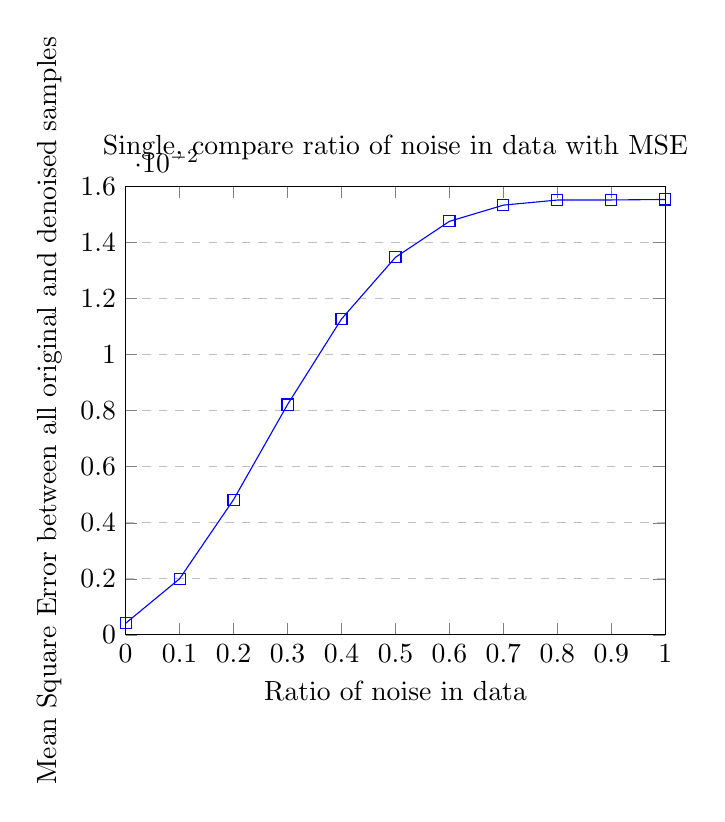
\begin{tikzpicture}
\begin{axis}[
    title={Single, compare ratio of noise in data with MSE},
    xlabel={Ratio of noise in data},
    ylabel={Mean Square Error between all original and denoised samples},
    xmin=0, xmax=1,
    ymin=0, ymax=0.016,
    xtick={0.0,0.1,0.2,0.3,0.4,0.5,0.6,0.7,0.8,0.9,1.0},
    ytick={0,0.002,0.004,0.006,0.008,0.01,0.012,0.014,0.016},
    legend pos=north west,
    ymajorgrids=true,
    grid style=dashed,
]
 
\addplot[
    color=blue,
    mark=square,
    ]
    coordinates {
    (0.0,0.00041424169804861347)
(0.1,0.0020027387880862716)
(0.2,0.004827114002054091)
(0.3,0.008219787743923315)
(0.4,0.011273536460116397)
(0.5,0.013474837384457377)
(0.6,0.014758644299897294)
(0.7,0.015337213283122217)
(0.8,0.015518657993837726)
(0.9,0.015522081478945567)
(1.0,0.015539198904484765)
    };

 
\end{axis}
\end{tikzpicture}

\npdecimalsign{.}
\nprounddigits{2}
\begin{tabu} to 0.8\textwidth { | X[l] | X[r] |}
\hline
samples &  MSE\\
\hline
292 & 0.08272412272456982\\
\hline
584 & 0.05112462867959078\\
\hline
876 & 0.038387678670901024\\
\hline
1168 & 0.030864036402654504\\
\hline
1460 & 0.025826996187060473\\
\hline
1752 & 0.022203898153853194\\
\hline
2044 & 0.019425278559739887\\
\hline
2336 & 0.01725685870494261\\
\hline
2628 & 0.015513051376325396\\
\hline
2921 & 0.014097320884351065\\
\hline
\end{tabu}
\npnoround



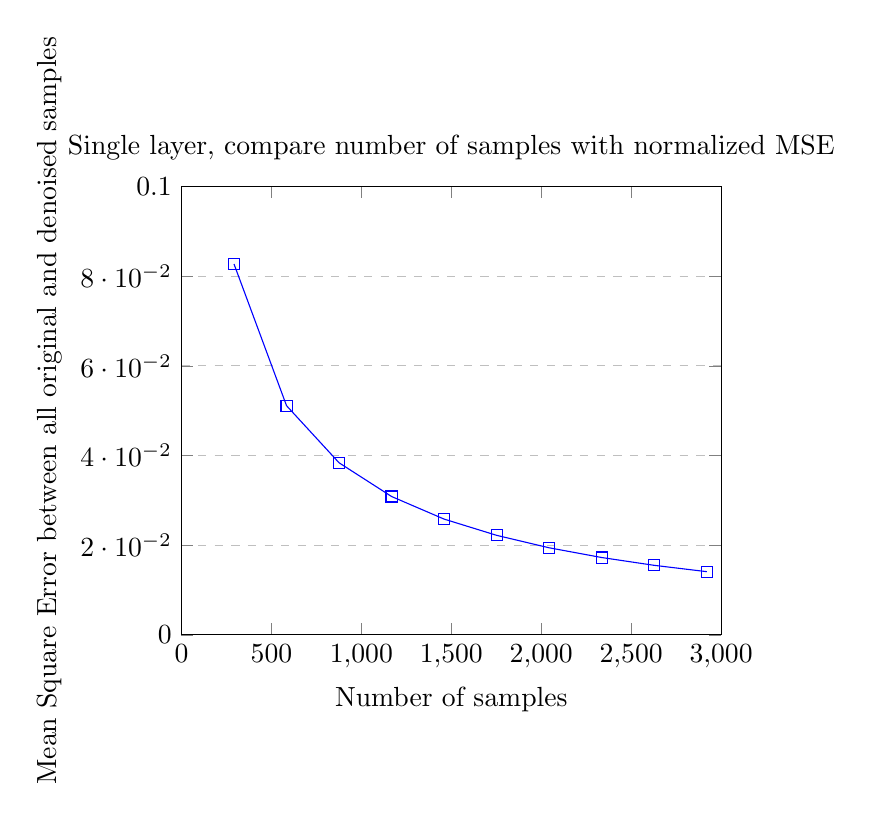
\begin{tikzpicture}
\begin{axis}[
    title={Single layer, compare number of samples with normalized MSE},
    xlabel={Number of samples},
    ylabel={Mean Square Error between all original and denoised samples},
    xmin=0, xmax=3000,
    ymin=0, ymax=0.1,
    xtick={0,500,1000,1500,2000,2500,3000},
    ytick={0,0.02,0.04,0.06,0.08,0.1},
    legend pos=north west,
    ymajorgrids=true,
    grid style=dashed,
]
 
\addplot[
    color=blue,
    mark=square,
    ]
    coordinates {
(292, 0.08272412272456982)
(584, 0.05112462867959078)
(876, 0.038387678670901024)
(1168, 0.030864036402654504)
(1460, 0.025826996187060473)
(1752, 0.022203898153853194)
(2044, 0.019425278559739887)
(2336, 0.01725685870494261)
(2628, 0.015513051376325396)
(2921, 0.014097320884351065)
    };
%    \legend{CuSO$_4\cdot$5H$_2$O}
 
\end{axis}
\end{tikzpicture}




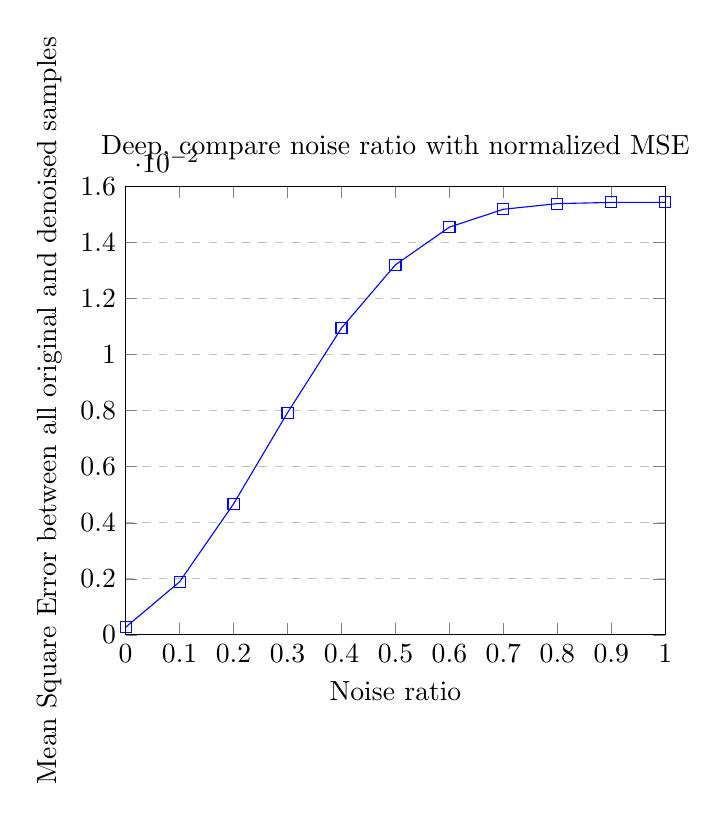
\begin{tikzpicture}
\begin{axis}[
    title={Deep, compare noise ratio with normalized MSE},
    xlabel={Noise ratio},
    ylabel={Mean Square Error between all original and denoised samples},
    xmin=0, xmax=1.0,
    ymin=0, ymax=0.016,
    xtick={0.0,0.1,0.2,0.3,0.4,0.5,0.6,0.7,0.8,0.9,1.0},
    ytick={0,0.002,0.004,0.006,0.008,0.01,0.012,0.014,0.016},
    legend pos=north west,
    ymajorgrids=true,
    grid style=dashed,
]
 
\addplot[
    color=blue,
    mark=square,
    ]
    coordinates {
(0.0, 0.00027164222900200914)
(0.1, 0.00189489109711971)
(0.2, 0.0046760299205644545)
(0.3, 0.007929749614054977)
(0.4, 0.010951344588837507)
(0.5, 0.013207739984301248)
(0.6, 0.014552935481772089)
(0.7, 0.015189768111575276)
(0.8, 0.015391140771116188)
(0.9, 0.015434603926379981)
(1.0, 0.01543832042568718)
    };
%    \legend{CuSO$_4\cdot$5H$_2$O}
 
\end{axis}
\end{tikzpicture}


\npdecimalsign{.}
\nprounddigits{2}
\begin{tabu} to 0.8\textwidth { | X[l] | X[r] |}
\hline
Noise ratio &  MSE\\
\hline
0.0 & 0.00027164222900200914\\
\hline
0.1 & 0.00189489109711971\\
\hline
0.2 & 0.0046760299205644545\\
\hline
0.3 & 0.007929749614054977\\
\hline
0.4 & 0.010951344588837507\\
\hline
0.5 & 0.013207739984301248\\
\hline
0.6 & 0.014552935481772089\\
\hline
0.7 & 0.015189768111575276\\
\hline
0.8 & 0.015391140771116188\\
\hline
0.9 & 0.015434603926379981\\
\hline
1.0 & 0.01543832042568718\\
\hline

\end{tabu}
\npnoround


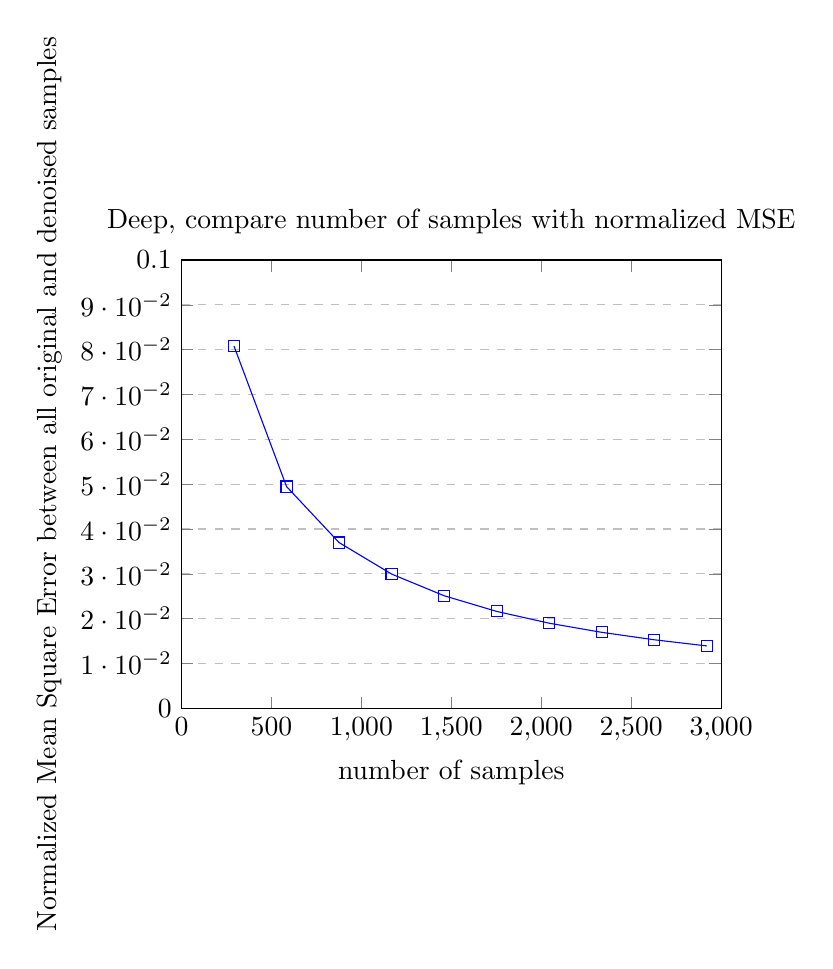
\begin{tikzpicture}
\begin{axis}[
    title={Deep, compare number of samples with normalized MSE},
    xlabel={number of samples},
    ylabel={Normalized Mean Square Error between all original and denoised samples},
    xmin=0, xmax=3000,
    ymin=0, ymax=0.1,
    xtick={0,500,1000,1500,2000,2500,3000},
    ytick={0,0.01,0.02,0.03,0.04,0.05,0.06,0.07,0.08,0.09,0.1},
    legend pos=north west,
    ymajorgrids=true,
    grid style=dashed,
]
 
\addplot[
    color=blue,
    mark=square,
    ]
    coordinates {
(292, 0.08079963129248201)
(584, 0.04946857863462037)
(876, 0.036976874680623634)
(1168, 0.029951494017716167)
(1460, 0.025115212164152242)
(1752, 0.021621704232002097)
(2044, 0.018989762754500344)
(2336, 0.01695257326686649)
(2628, 0.015293442879119832)
(2921, 0.01391785980540682)
    };
%    \legend{CuSO$_4\cdot$5H$_2$O}
 
\end{axis}
\end{tikzpicture}



\npdecimalsign{.}
\nprounddigits{2}
\begin{tabu} to 0.8\textwidth { | X[l] | X[r] |}
\hline
Samples &  Normalized MSE\\
\hline
292 & 0.08079963129248201\\
\hline
584 & 0.04946857863462037\\
\hline
876 & 0.036976874680623634\\
\hline
1168 & 0.029951494017716167\\
\hline
1460 & 0.025115212164152242\\
\hline
1752 & 0.021621704232002097\\
\hline
2044 & 0.018989762754500344\\
\hline
2336 & 0.01695257326686649\\
\hline
2628 & 0.015293442879119832\\
\hline
2921 & 0.01391785980540682\\
\hline
\end{tabu}
\npnoround


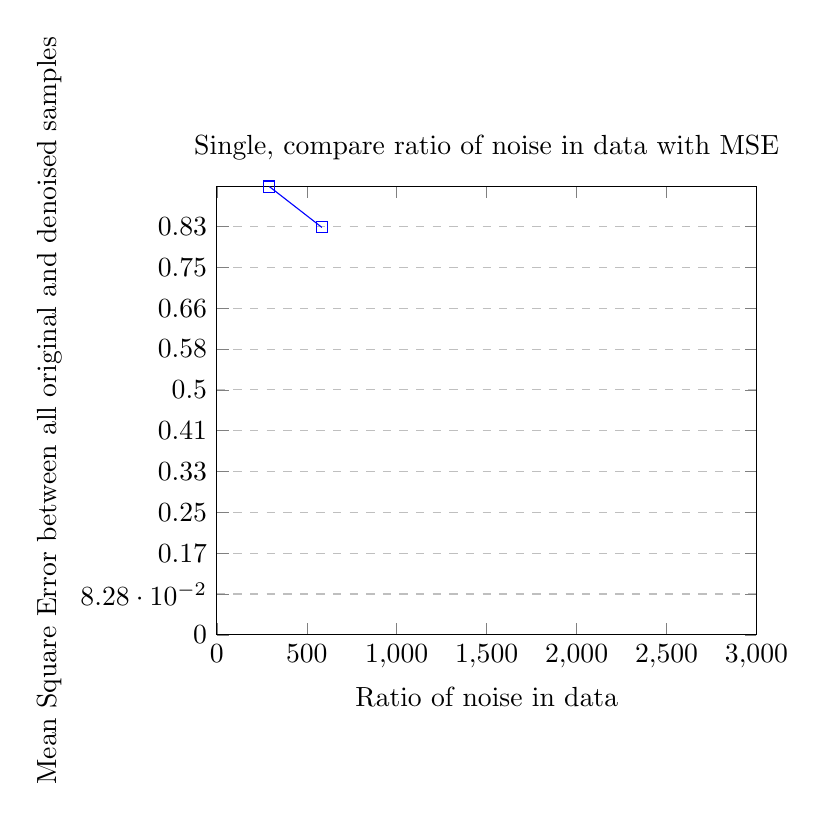
\begin{tikzpicture}
\begin{axis}[
title={Single, compare ratio of noise in data with MSE},
xlabel={Ratio of noise in data},
ylabel={Mean Square Error between all original and denoised samples},
xmin=0, xmax=3000,
ymin=0, ymax=0.9090955376510923,
xtick={0,500,1000,1500,2000,2500,3000},
ytick={0,0.08279400680556004,0.16558801361112008,0.24838202041668012,0.33117602722224015,0.4139700340278002,0.49676404083336023,0.5795580476389203,0.6623520544444803,0.7451460612500403,0.8279400680556004},
legend pos=north west,
ymajorgrids=true,
grid style=dashed,
]

\addplot[
color=blue,
mark=square,
]
coordinates {

(292, 0.9090955376510923)
(584, 0.8263015308455323)
    };
\end{axis}
\end{tikzpicture}

\npdecimalsign{.}
\nprounddigits{2}
\begin{tabu} to 0.8\textwidth { | X[l] | X[r] |}
\hline
samples &  MSE\\
\hline
292 & 0.9090955376510923\\
\hline
584 & 0.8263015308455323\\
\hline
\end{tabu}
\npnoround





\end{document}